\documentclass[11pt]{article}
\title{\textbf{Meccano nonagon}}
\author{https://github.com/heptagons/meccano/nona}
\date{}

\usepackage{../meccano}

%\usepackage{amsmath}
%\usepackage[pdftex]{graphicx}

\begin{document}

\maketitle

\begin{figure}[h]
\centering
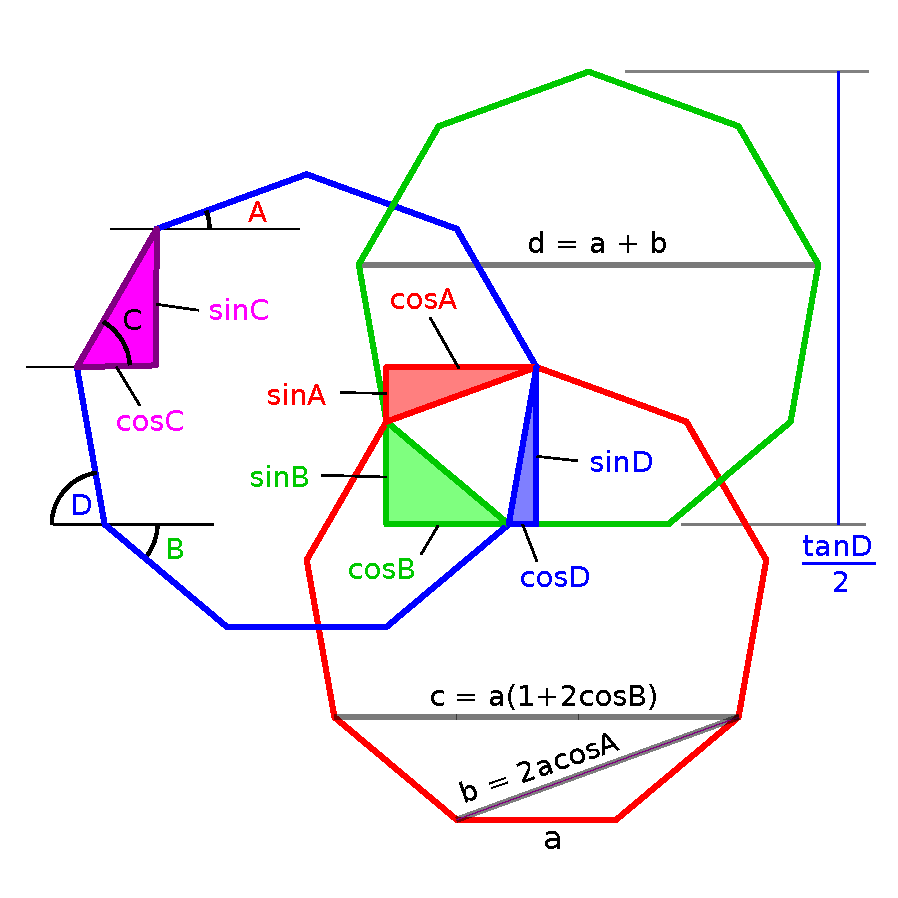
\includegraphics[scale=0.7]{figs/3nonagons}
\caption{Three regular nonagons connected by an equilateral triangle.
We note four angles in the figure $A$, $B$, $C$ and $D$.}
\label{fig:nonagons}
\end{figure}

\section{Algebra}

Figure \ref{fig:nonagons} shows three regular nonagons connected by an equilateral 
triangle. Four angles appear orthogonally in any regular nonagon:
\begin{align}
A &= \pi/9 = 20^{\circ} \\
B &= 2\pi/9 = 40^{\circ} \\
C &= 3\pi/9 = 60^{\circ} \\
D &= 4\pi/9 = 80^{\circ} \\
A + B &= D - A = C
\end{align}

The relations of angle $C$ are those of equilateral triangle:
\begin{align}
\cos{C} &= -\frac{1}{2}\\
\sin{C} &= \frac{\sqrt{3}}{2}
\end{align}

From the figure \ref{fig:nonagons}, cosines of angles $A$, $B$ and $D$ are related as:
\begin{align}
\cos{A} &= \cos{B} + \cos{D} \\
 &= \cos{(2A)} + \cos{(4A)} \nonumber\\
 &= (2\cos^2{A} - 1) + (1 -8\cos^2{A} + 8\cos^4{A}) \nonumber\\
 &= 8\cos^4{A} - 6\cos^2{A} \nonumber\\
 1 &= 8\cos^3{A} - 6\cos{A}
\end{align}

Previous cosines equation is the depressed cubic equation:
\begin{align}
t^3 +pt +q &= 0 \label{eq:cubic}\\
p &= -\frac{3}{4}\\
q &= -\frac{1}{8}
\end{align}
We found the discriminant is negative which means we have three real roots:
\begin{align}
\Delta &= \frac{q^2}{4} + \frac{p^3}{27} = -\frac{3}{64} \nonumber\\
t_k &= 2\sqrt{-\frac{p}{3}}\cos\left({\frac{1}{3}\arccos\left(
\frac{3q}{2p}\sqrt{\frac{-3}{p}}
\right) -k\frac{2\pi}{3}}\right) &\texttt{for } k=0,1,2. \nonumber\\
&= \cos\left(\frac{1}{3}\arccos\left(\frac{1}{2}\right) -k\frac{2\pi}{3} \right)  &\texttt{for } k=0,1,2. \nonumber\\
&= \cos\left(\frac{1}{3}\left(\frac{\pi}{3}\right) -k\frac{2\pi}{3} \right)  &\texttt{for } k=0,1,2. \nonumber\\
t_0 &= \cos\left(\frac{\pi}{9}\right) = \cos{A} \approx +0.939692\\
t_1 &= \cos\left(-\frac{2\pi}{9}\right) = -\cos{B} \approx -0.766044 \\
t_2 &= \cos\left(-\frac{4\pi}{9}\right) = -\cos{D} \approx -0.173648
\end{align}

From equation \ref{eq:cubic} we know the product of roots squares is $-2p = \frac{3}{2}$:
\begin{align}
\cos^2{A} + \cos^2{B} + \cos^2{D} &= \frac{3}{2} \\
1 - \sin^2{A} + 1 - \sin^2{B} + 1 - \sin^2{D} &= \frac{3}{2} \nonumber\\
\sin^2{A} + \sin^2{B} + \sin^2{D} &= \frac{3}{2}
\end{align}

From equation \ref{eq:cubic} we know the product of roots is $-q = \frac{1}{8}$ matching the ``Morrie's law'':
\begin{align}
\cos{A}\cos{B}\cos{D} &= \frac{1}{8} \\
(1-\sin^2{A})(1-\sin^2{B})(1-\sin^2{D}) &= \frac{1}{64} \nonumber\\
(\sin{A}\sin{B})^2 +(\sin{A}\sin{D})^2 +(\sin{C}\sin{D})^2 &= \frac{1}{64} - 1 +\sin^2{A}+\sin^2{B}+\sin^2{D} +(\sin{A}\sin{B}\sin{D})^2 \nonumber\\
 &= \frac{1}{64} - 1 + \frac{3}{2} +\left(\frac{\sqrt{3}}{8}\right)^2 = \left(\frac{9}{4}\right)^2 
\end{align}

From the figure \ref{fig:nonagons}, sines of angles $A$, $B$ and $D$ are related as:
\begin{align}
\sin{A} + \sin{B} &= \sin{D} \\
 &= \sin(2A + B) \nonumber\\
 &= \sin(2A)\cos{B} + \cos(2A)\sin{B} \nonumber\\
 &= 2\sin{A}\cos{A}\cos{B} + (1-2\sin^2{A})\sin{B} \nonumber\\
\sin{A} &= 2\sin{A}\cos{A}\cos{B} -2\sin^2{A}\sin{B} \nonumber\\
1 &= 2\cos{A}\cos{B} -2\sin{A}\sin{B} \\
  &= 2\cos(A+B) = 2\cos{C} \nonumber
\end{align}

Nonagon height is sum of all sines:
\begin{align}
\sin{A}+\sin{B}+\sin{C}+\sin{D} &= 2\sin{D} + \frac{\sqrt{3}}{2}
\end{align}



Last equation solves this cubic equation:
\begin{align*}
y^3 - \frac{3y}{4} - \frac{3}{8} &= 0\\
y_1 &= -\sin{A} \approx -0.342020\\
y_2 &= -\sin{B} \approx -0.642787\\
y_3 &= +\sin{C} \approx +0.984807
\end{align*}

More sines relations of angles $A$, $B$ and $C$ are:
\begin{align*}
\sin{A}\sin{B}\sin{C} &= \frac{\sqrt{3}}{8}\\
\sin^2{A} + \sin^2{B} + \sin^2{C} &= \frac{3}{2}
\end{align*}

Cosines and sines relations are:
\begin{align*}
\cos{A}\cos{B} - \sin{A}\sin{B} &= \frac{1}{2}\\
\frac{1}{\cos{C}} -\frac{\sqrt{3}}{\sin{C}} &= 4\\
\tan{C} - 4\sin{C} &= \sqrt{3}
\end{align*}

\end{document}
